\section{V4 et V5 : auto-apprentissage transductif}\label{sec:selftrain}

Après la V3, chaque brique transductive (équilibrage, alignement, voisins) agissait \emph{au moment de la prédiction} : le modèle restait celui de la période d'entraînement, et l'on corrigeait ses sorties. L'auto-apprentissage va plus loin : il \emph{réentraîne} le modèle sur des fenêtres de la période test, étiquetées par un modèle précédent. C'est l'idée du \emph{pseudo-label}~\cite{lee} et de l'élève bruité~\cite{xie}, appliquée ici à un changement de période plutôt qu'à des données non étiquetées de même loi. Deux tours ont été joués. Le premier (V4) prend V3~B comme professeur, le second (V5) prend V4~C. Ils font passer le score public de $0{,}6351$ à $\mathbf{0{,}6835}$, soit le plus gros gain cumulé du projet après la représentation initiale.

\begin{figure}[H]\centering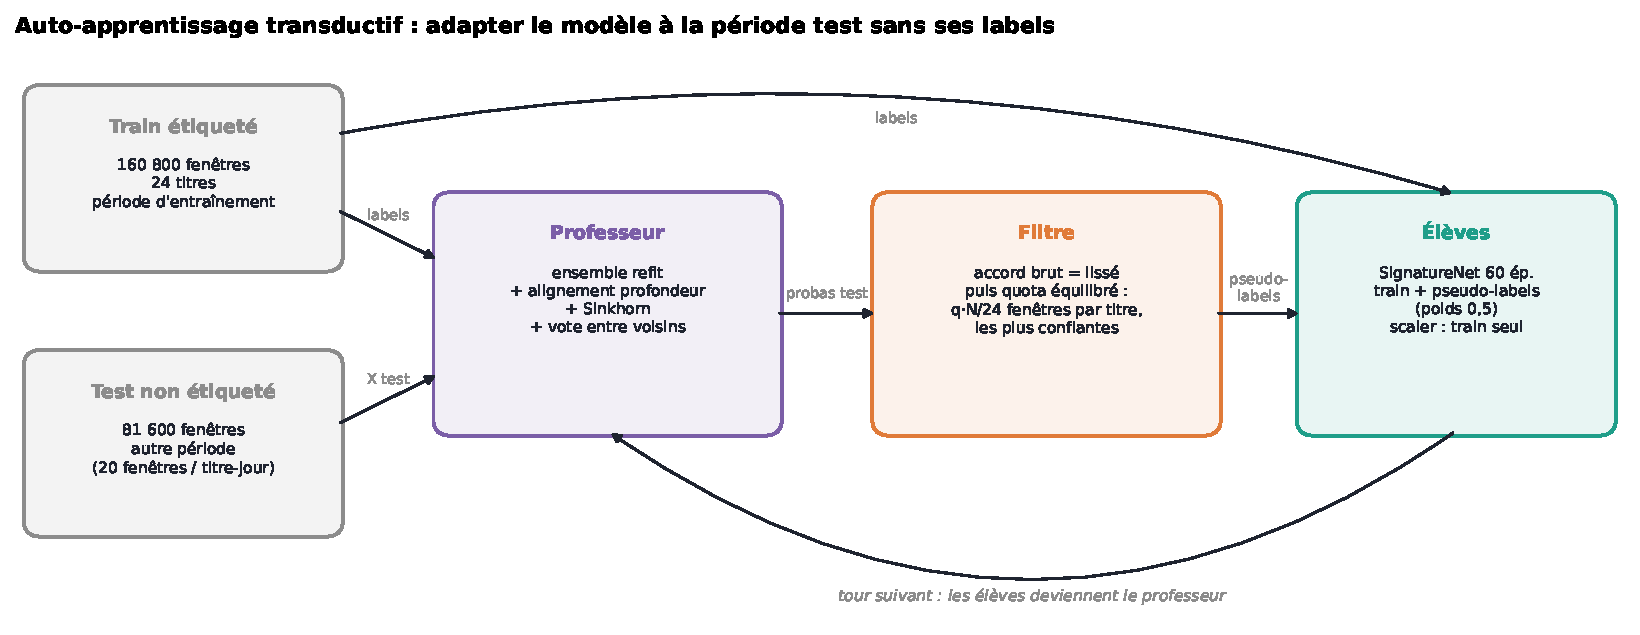
\includegraphics[width=\linewidth]{figures/v5_self_training_loop.pdf}
\caption{La boucle d'auto-apprentissage. Le professeur étiquette les fenêtres test où ses deux lectures concordent ; un quota par titre empêche de transmettre son biais de classes ; les élèves s'entraînent sur train $\cup$ pseudo-labels, puis deviennent le professeur du tour suivant.}
\label{fig:loop}\end{figure}

\subsection{Formalisation}

\paragraph{Les deux lectures du professeur.} Soit $\mathcal{T}$ l'ensemble des $N=81\,600$ fenêtres test. Le professeur fournit deux matrices de probabilités sur $\mathcal{T}$ :
\begin{itemize}
\item la lecture \emph{brute} $P^{\text{brut}}=\mathrm{Sinkhorn}\big(\tfrac1M\sum_{m}P^{(m)}\big)$, moyenne équilibrée de ses $M$ membres ;
\item la lecture \emph{lissée} $Q=\mathrm{Sinkhorn}\big(Q^{(5)}\big)$, après le vote entre voisins de la section~\ref{sec:voisins}. C'est la soumission elle-même.
\end{itemize}
On note $\hat y_i=\arg\max_c Q_{ic}$ et $\kappa_i=\max_c Q_{ic}$ la confiance.

\begin{definition}[Fenêtres éligibles]
$\mathcal{E}=\{i\in\mathcal{T} : \arg\max_c Q_{ic}=\arg\max_c P^{\text{brut}}_{ic}\}$.
\end{definition}
\noindent Les deux lectures n'utilisent pas la même information. $P^{\text{brut}}$ ne regarde que la fenêtre $i$. $Q$ regarde aussi ses voisines du même titre-jour. Exiger leur accord revient à demander deux « vues » concordantes, dans l'esprit du co-apprentissage~\cite{blum} : une fenêtre dont le label ne tient qu'au vote de ses voisines, ou qu'à sa seule lecture isolée, est écartée. Le désaccord touche 9,1\,\% du test en V4 et 7,9\,\% en V5.

\begin{definition}[Quota équilibré]
Pour une part $q\in(0,1)$, soit $m=\lfloor qN/K\rfloor$. Pour chaque titre $c$, on retient les $m$ fenêtres de $\mathcal{E}\cap\{\hat y=c\}$ de plus grande confiance $\kappa_i$ :
\begin{equation}
\mathcal{S}_q=\bigcup_{c=1}^{K}\operatorname{top}_m\big(\{i\in\mathcal{E} : \hat y_i=c\},\ \kappa\big).
\end{equation}
\end{definition}

\begin{remarque}[Pourquoi un quota plutôt qu'un seuil]
Un seuil $\kappa_i\ge\tau$ retient davantage de fenêtres dans les titres faciles. Le prior empirique des pseudo-labels hérite alors du biais du professeur, et l'élève le renforce. Avec le quota, $|\mathcal{S}_q\cap\{\hat y=c\}|=m$ pour tout $c$, dès que chaque titre a au moins $m$ fenêtres éligibles. C'est le cas dans les deux tours : en V5, le titre le moins fourni compte 2\,795 éligibles pour un quota de 2\,040 à $q=0{,}6$. Le prior des pseudo-labels est donc exactement uniforme, ce qui est cohérent avec l'hypothèse d'un test équilibré déjà utilisée par Sinkhorn (section~\ref{sec:sinkhorn}).
\end{remarque}

\paragraph{Emboîtement.} Comme la sélection se fait par confiance décroissante à l'intérieur de chaque titre, $q<q'\Rightarrow\mathcal{S}_q\subseteq\mathcal{S}_{q'}$. Le contrôle $q=0{,}4$ de la V5 est donc un sous-ensemble strict de la sélection $q=0{,}6$ : les deux élèves ne diffèrent que par les 16\,320 fenêtres les moins sûres.

\paragraph{Perte de l'élève.} Soit $\mathcal{D}$ les fenêtres étiquetées utilisées pour l'entraînement (le fit en développement, tous les labels au refit). L'élève minimise, sur chaque lot $B\subset\mathcal{D}\cup\mathcal{S}_q$, la moyenne pondérée
\begin{equation}
\mathcal{L}_B(\theta)=\frac{\sum_{j\in B}w_j\,\ell_\varepsilon\big(f_\theta(x_j),\tilde y_j\big)}{\sum_{j\in B}w_j},\qquad
(w_j,\tilde y_j)=\begin{cases}(1,\,y_j) & j\in\mathcal{D}\\ (\omega,\,\hat y_j) & j\in\mathcal{S}_q\end{cases}
\end{equation}
où $\ell_\varepsilon$ est l'entropie croisée avec lissage des labels et $\omega=0{,}5$. Deux garde-fous complètent la formule. La standardisation du contexte est estimée sur les seules fenêtres étiquetées, pour que les statistiques du test n'entrent pas par ce biais. Le fichier de pseudo-labels est vérifié par empreinte et par alignement sur les \code{obs\_id} du test : un run ne peut pas être réutilisé avec d'autres pseudo-labels.

\begin{algo}[H]
\caption{Un tour d'auto-apprentissage}\label{alg:selftrain}
\begin{algobox}
\item Entrées : probabilités brute $P^{\text{brut}}$ et lissée $Q$ du professeur sur le test ; part $q$ ; poids $\omega$.
\item $\mathcal{E}\leftarrow\{i : \arg\max Q_i=\arg\max P^{\text{brut}}_i\}$.
\item Pour chaque titre $c$ : garder les $\lfloor qN/K\rfloor$ fenêtres de $\mathcal{E}$ prédites $c$ de plus grande confiance $\Rightarrow\mathcal{S}_q$, labels $\hat y$.
\item Entraîner $S$ graines de SignatureNet (60 époques, configuration \code{v3\_long}) sur fit $\cup\,\mathcal{S}_q$ ; sélectionner l'époque sur valid.
\item Refit de chaque graine sur tous les labels $\cup\,\mathcal{S}_q$, même nombre d'époques.
\item Prédire le test, alignement de profondeur si adopté, moyenne, vote entre voisins, Sinkhorn $\Rightarrow$ nouveau $Q$.
\item Le nouvel ensemble devient le professeur du tour suivant.
\end{algobox}
\end{algo}

\subsection{La mesure interne est contaminée}\label{sec:contam}
\begin{proposition}
Les précisions valid et stress d'un élève sont biaisées vers le haut par rapport à celles d'un modèle sans pseudo-labels, indépendamment de tout gain de transfert.
\end{proposition}
\begin{proof}[Argument]
Le professeur est un ensemble \emph{refit}, entraîné sur tous les labels, valid et stress compris. Ses pseudo-labels $\hat y$ sont donc des fonctions de $y_{\text{valid}}$ et $y_{\text{stress}}$. En apprenant $\hat y$ sur des fenêtres test proches des fenêtres valid (même titre, régime voisin), l'élève reçoit indirectement une partie de l'information de leurs labels. Son score valid n'est plus celui d'un modèle qui n'a jamais vu ces labels.
\end{proof}
\noindent L'ampleur du biais est inconnue. Elle croît avec $q$ : plus de pseudo-labels transmettent plus d'information. Conséquence pratique : dans cette section, les mesures internes servent à vérifier que l'entraînement s'est bien passé. Les gains se lisent \emph{uniquement} au LB, à l'aide de soumissions de contrôle qui ne diffèrent que d'un élément.

\subsection{V4 : le premier tour et son contrôle}
\paragraph{Pseudo-labels.} Le professeur est V3~B (0,6351). Ses lectures brute (V3~A) et lissée concordent sur 90,9\,\% du test. Avec $q=0{,}4$, on retient 32\,640 fenêtres, 1\,360 par titre, de confiance moyenne 0,813 et minimale 0,455.

\begin{table}[H]\centering\small
\begin{tabular}{lcccc}
\toprule
Configuration & Graines & Valid éq. & Stress éq. & Meilleure époque\\
\midrule
\code{v3\_long} (ancre, 60 époques) & 2 & 0,785 & 0,791 & 54--58\\
\code{v4\_xlong} (90 époques) & 3 & 0,797 & 0,800 & 55--90\\
\code{v4\_student} (\code{v3\_long} + pseudo-labels, $q=0{,}4$) & 2 & \textbf{0,814} & \textbf{0,815} & 49--59\\
\bottomrule
\end{tabular}
\caption{V4, modèles seuls (Sinkhorn appliqué à chacun). Les élèves sont en partie contaminés (section~\ref{sec:contam}).}
\end{table}

\begin{table}[H]\centering\small
\begin{tabular}{llc}
\toprule
Soumission & Contenu & LB public\\
\midrule
V3 B (référence) & 6 modèles à 60 époques, alignement, Sinkhorn, voisins & 0,6351\\
\textbf{V4 C} & \code{v4\_xlong} $\times3$ + élèves $\times2$, $\gamma=1{,}239$, Sinkhorn, voisins ($k=40$) & \textbf{0,6551}\\
V4 D (contrôle) & \code{v4\_xlong} $\times3$ seuls, mêmes post-traitements & \old{0,6174}\\
\bottomrule
\end{tabular}
\caption{Le contrôle D isole les élèves. C $-$ D $=+3{,}8$ points : tout le gain de la V4 leur revient.}
\end{table}

\paragraph{Deux lectures du contrôle.}
\begin{enumerate}
\item \textbf{L'entraînement long ne transfère pas.} En interne, 90 époques gagnent $+1{,}1$ point sur 60. Au LB, D est $1{,}8$ point \emph{sous} V3~B. C'est la première fois dans le projet qu'un gain interne change de signe au LB. Deux causes restent confondues : le surapprentissage de la période d'entraînement (figure~\ref{fig:curves}, la log-loss valid de \code{v4\_xlong} ne baisse plus après l'époque 40) et un ensemble deux fois plus petit (3 modèles contre 6).
\item \textbf{Les élèves corrigent les fenêtres qu'on ne leur a pas données.} C et D sont d'accord sur 98,9\,\% des fenêtres pseudo-étiquetées, mais sur 81,5\,\% seulement des 60\,\% restantes. Le gain de C ne vient donc pas d'une copie du professeur. Les élèves ont appris des traits propres à la période test et les ont étendus aux fenêtres les plus difficiles. C'est de l'adaptation de domaine.
\end{enumerate}

\subsection{V5 : un second tour, un meilleur professeur}
\paragraph{Hypothèses, fixées avant le run.} H1 : un professeur meilleur (V4~C, 0,6551) donne de meilleurs pseudo-labels, donc de meilleurs élèves. H2 : passer de $q=0{,}4$ à $q=0{,}6$ donne plus de signal sur la période test. Ce signal porte sur les fenêtres non étiquetées, là où la V4 a gagné. Les modèles longs sont abandonnés.

\paragraph{Pseudo-labels.} Les lectures brute et lissée de V4~C concordent sur 92,1\,\% du test.
\begin{table}[H]\centering\small
\begin{tabular}{lccccc}
\toprule
Quota & Fenêtres & Par titre & Titres sous le quota & Confiance min. & Confiance moy.\\
\midrule
$q=0{,}4$ & 32\,640 & 1\,360 & 0 & 0,544 & 0,849\\
$q=0{,}6$ & 48\,960 & 2\,040 & 0 & 0,456 & 0,791\\
\bottomrule
\end{tabular}
\caption{Sélections V5. Elles sont emboîtées : la sélection à 40\,\% est incluse dans celle à 60\,\%.}
\end{table}

\begin{figure}[H]\centering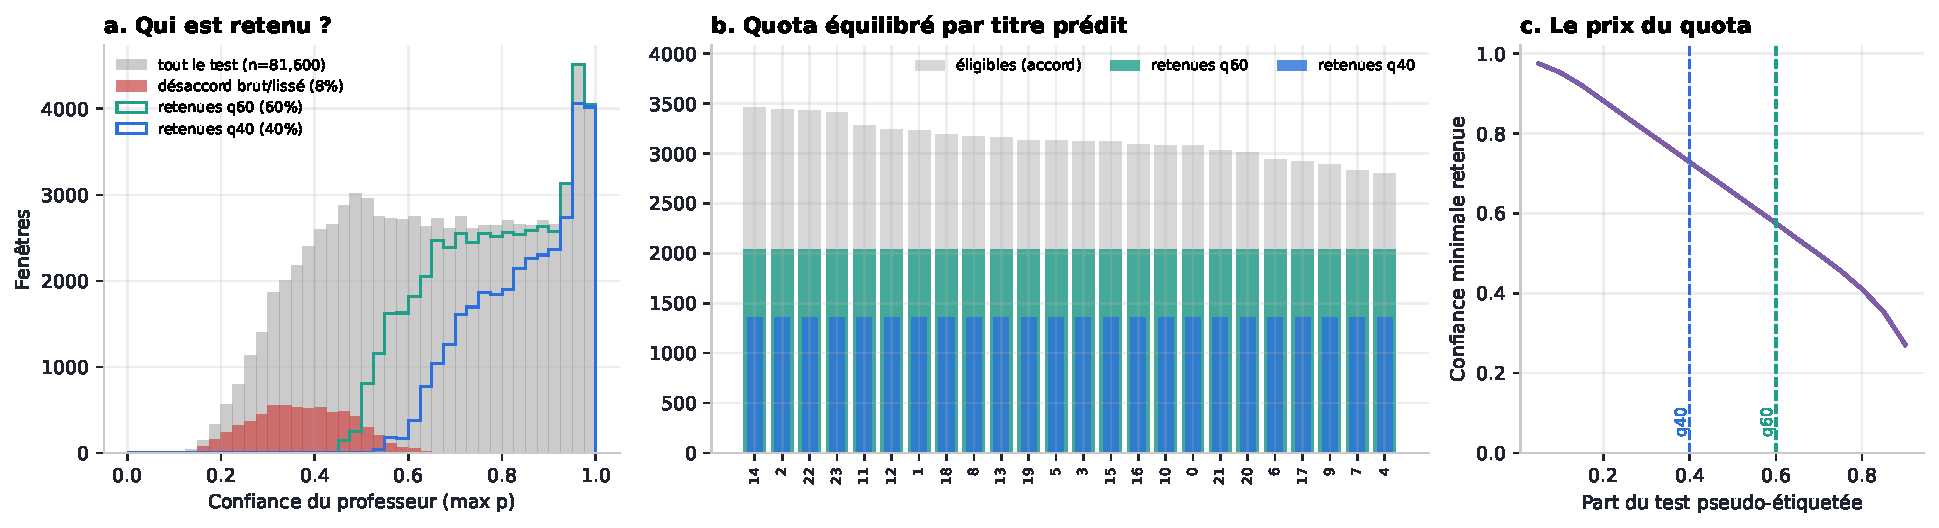
\includegraphics[width=\linewidth]{figures/v5_pseudo_selection.pdf}
\caption{Sélection des pseudo-labels V5. (a) Les fenêtres où les deux lectures divergent ont une confiance faible (mode vers 0,3) : le filtre écarte bien les cas douteux. (b) Le quota coupe les titres sur-prédits : chaque titre reçoit exactement 2\,040 (resp. 1\,360) fenêtres. (c) Confiance minimale atteinte si l'on étendait la sélection sans quota. Elle chute rapidement au-delà de 60\,\%, ce qui borne l'intérêt d'aller plus loin.}
\label{fig:pseudo}\end{figure}

\paragraph{Élèves.}
\begin{table}[H]\centering\small
\begin{tabular}{lccccc}
\toprule
Configuration & Graines & Valid éq. & Stress éq. & Accord test avec V4 C & Minutes\\
\midrule
\code{v5\_q40} & 3 & 0,813 $\pm$ 0,003 & 0,815 $\pm$ 0,001 & 0,787 & 16,0\\
\code{v5\_q60} & 3 & \textbf{0,823} $\pm$ 0,000 & \textbf{0,826} $\pm$ 0,000 & 0,826 & 17,7\\
\bottomrule
\end{tabular}
\caption{V5, modèles seuls (moyenne $\pm$ écart-type entre graines). L'écart q60 $-$ q40 ($+1$ point) est compatible avec une contamination plus forte et ne prouve pas H2.}
\end{table}

\begin{figure}[H]\centering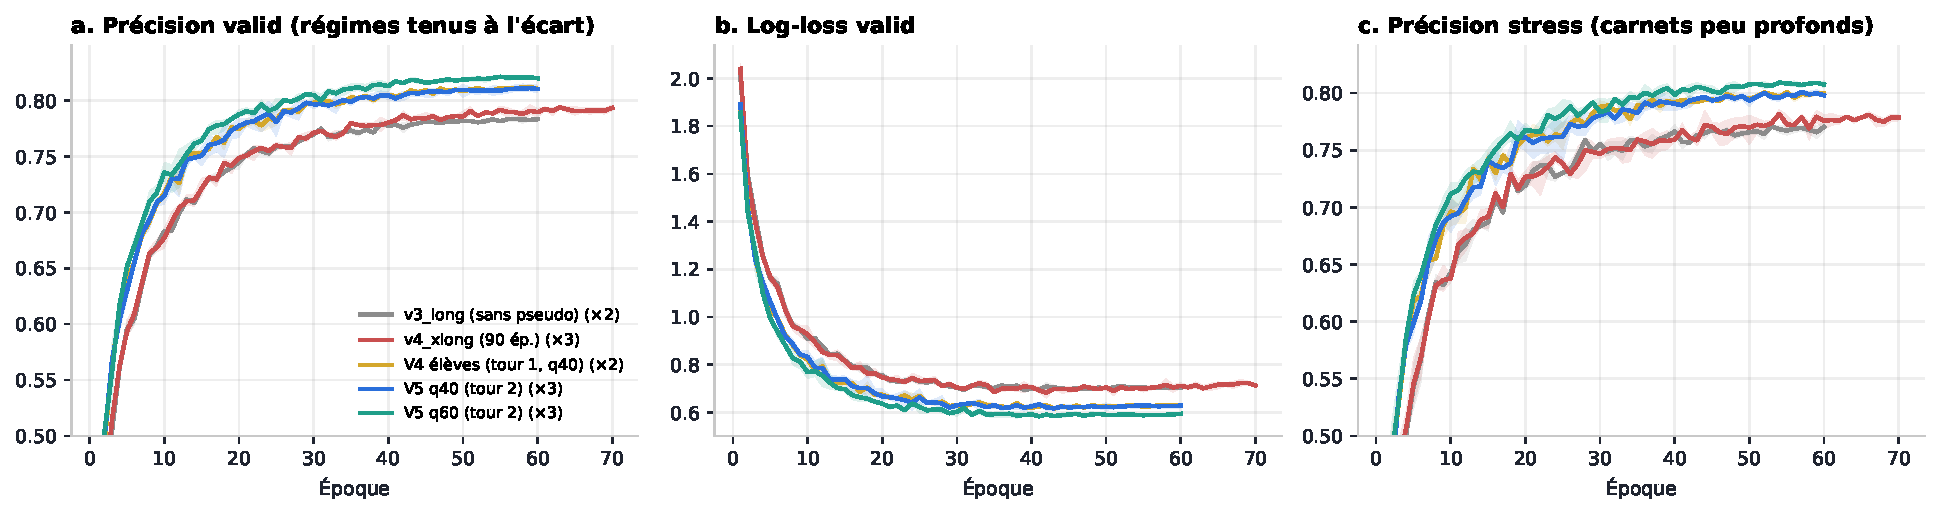
\includegraphics[width=\linewidth]{figures/v5_learning_curves_all.pdf}
\caption{Courbes d'apprentissage des trois générations (moyenne sur les graines ; bande = min/max). Les élèves des deux tours se séparent des modèles sans pseudo-labels dès les premières époques. Leur log-loss valid descend à 0,59--0,63 contre 0,70 et ne remonte pas. \code{v4\_xlong} rejoint \code{v3\_long} sans le dépasser nettement (la courbe s'arrête à 70 époques, l'arrêt précoce d'une graine).}
\label{fig:curves}\end{figure}

\begin{figure}[H]\centering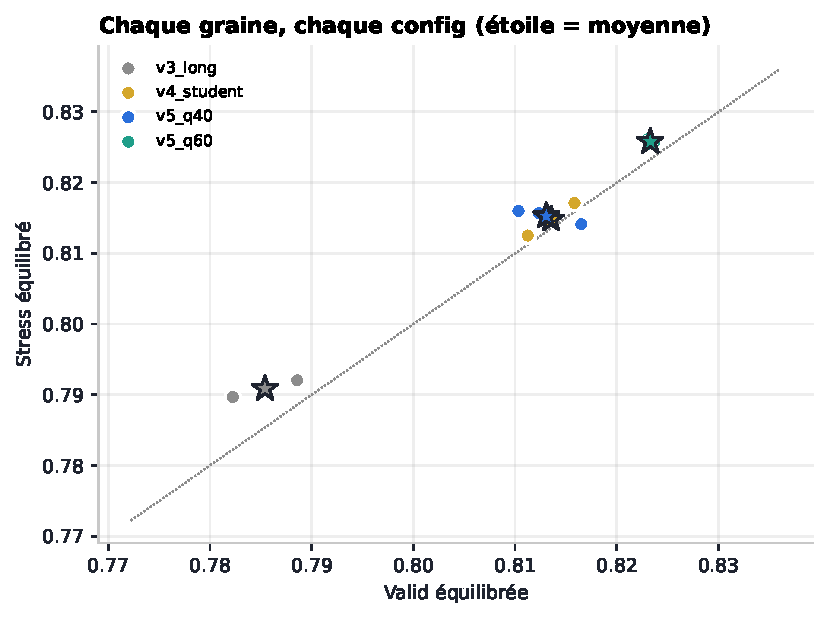
\includegraphics[width=.6\linewidth]{figures/v5_runs_all.pdf}
\caption{Chaque graine, en valid et en stress équilibrés. Les générations forment des grappes nettes, et la dispersion entre graines (moins de 0,5 point) est petite devant l'écart entre générations.}
\end{figure}

\paragraph{Ensemble et post-traitements.} L'alignement de profondeur n'apporte que $+0{,}2$ point en stress, sous le seuil de $+0{,}3$ fixé d'avance : il est rejeté, et $\gamma_{\text{test}}=1$ (contre 1,239 en V4). La cascade se lit sur le pool valid $\cup$ stress :
\begin{table}[H]\centering\small
\begin{tabular}{lcccc}
\toprule
Étape & V4 & V5 & $\Delta$ V5 vs V4\\
\midrule
Meilleur modèle seul & 0,808 & 0,818 & +1,0\\
Moyenne de l'ensemble & 0,830 & 0,842 & +1,2\\
+ Sinkhorn & 0,835 & 0,846 & +1,1\\
+ voisins (\code{combo}, $k=10$, $\alpha=0{,}5$, 5 it.) & 0,848 & 0,856 & +0,8\\
\midrule
Gain des voisins & +1,3 & +1,0 & \\
\bottomrule
\end{tabular}
\caption{Cascade interne (précision ; équilibrée à partir de Sinkhorn). Mesures contaminées : seule la forme de la cascade est informative.}
\end{table}
\noindent Les voisins rapportent moins en V5 : leurs pseudo-labels venaient d'un professeur déjà lissé, donc les élèves ont absorbé une partie de l'information du voisinage. La grille (figure~\ref{fig:nbr}) garde le même optimum qu'en V3 et V4 ($\alpha=0{,}5$, $k=10$), ce qui rend le passage à $k_{\text{test}}=40$ cohérent d'un tour à l'autre.

\begin{figure}[H]\centering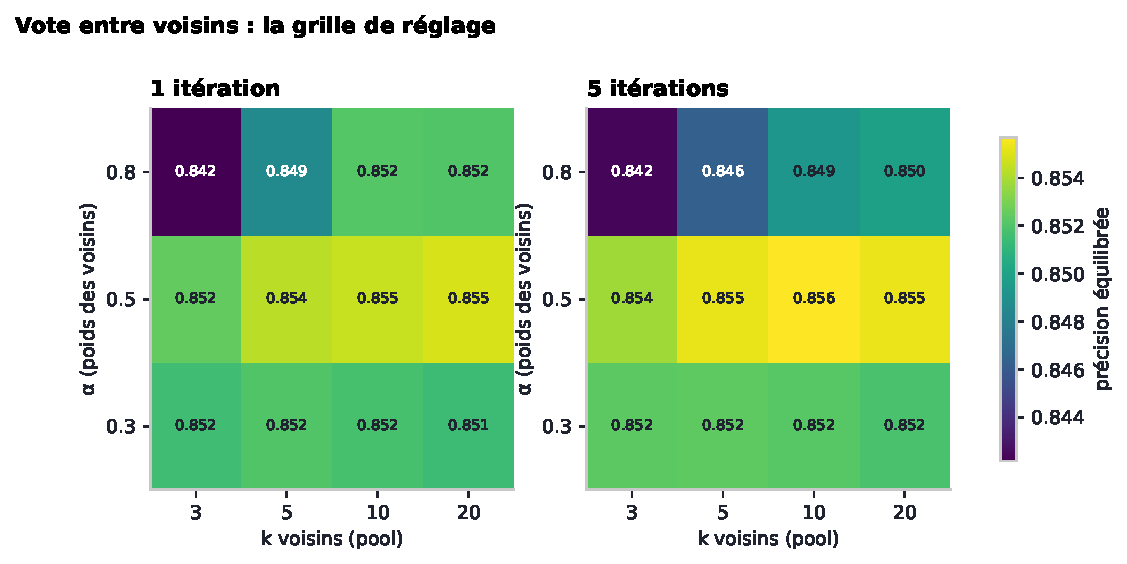
\includegraphics[width=.85\linewidth]{figures/v5_neighbours.pdf}
\caption{Grille du vote entre voisins sur le pool. Un $\alpha$ trop fort (0,8) dégrade d'autant plus que $k$ et le nombre d'itérations augmentent : le lissage écrase alors l'information propre à chaque fenêtre.}
\label{fig:nbr}\end{figure}

\subsection{Ce qui change au test, et le verdict du LB}
\begin{table}[H]\centering\small
\begin{tabular}{lccc}
\toprule
Soumission V5 & Différent de V4 C (total) & sur $\mathcal{S}_{0,6}$ (60\,\%) & hors $\mathcal{S}_{0,6}$ (40\,\%)\\
\midrule
ALL (6 élèves) & 11,2\,\% & 1,0\,\% & \textbf{26,5\,\%}\\
E (\code{v5\_q60} $\times3$) & 12,1\,\% & 0,8\,\% & 29,2\,\%\\
F (\code{v5\_q40} $\times3$) & 12,6\,\% & 2,0\,\% & 28,4\,\%\\
\bottomrule
\end{tabular}
\caption{Les élèves recopient le professeur là où ils ont été étiquetés, et modifient plus d'une fenêtre sur quatre ailleurs.}
\end{table}

\begin{figure}[H]\centering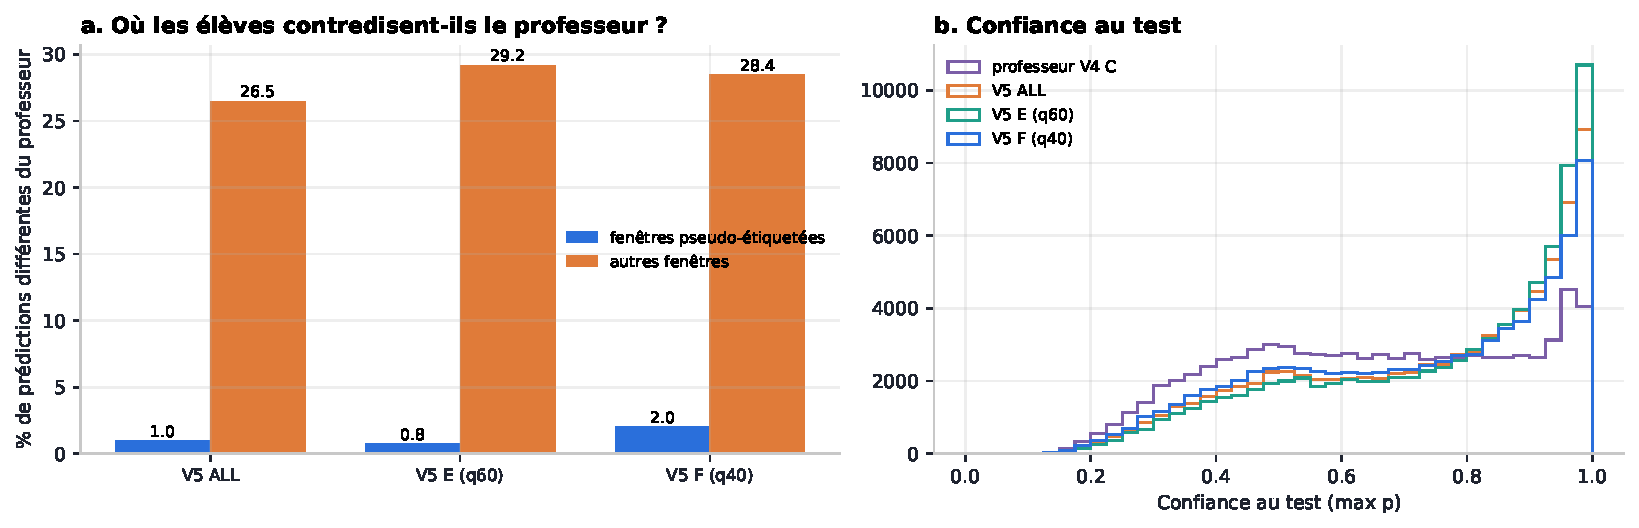
\includegraphics[width=\linewidth]{figures/v5_test_changes.pdf}
\caption{(a) Désaccords avec le professeur, sur et hors pseudo-labels. (b) Confiance au test. La masse du professeur, étalée entre 0,4 et 0,7, se concentre chez les élèves au-dessus de 0,9.}
\label{fig:testchg}\end{figure}

\begin{table}[H]\centering\small
\begin{tabular}{llc}
\toprule
Soumission & Contenu & LB public\\
\midrule
V4 C (professeur) & — & 0,6551\\
\textbf{V5 ALL} & 6 élèves, Sinkhorn, voisins ($k=40$) & \textbf{0,6835}\\
V5 E & \code{v5\_q60} $\times3$ seuls, mêmes post-traitements & 0,6822\\
V5 F & \code{v5\_q40} $\times3$ seuls & non soumise\\
\bottomrule
\end{tabular}
\caption{H1 est confirmée : $+2{,}8$ points sur le professeur. E fait presque aussi bien que ALL avec deux fois moins de modèles. H2 (E $-$ F) reste ouverte faute de soumission F.}
\end{table}

\paragraph{Le durcissement de la confiance n'est pas un mauvais calibrage.} La figure~\ref{fig:testchg}b est le symptôme classique du \emph{biais de confirmation}~\cite{arazo} : un élève entraîné sur ses propres certitudes devient plus sûr de lui. Mais sur le stress, les élèves sont \emph{mieux} calibrés que les modèles sans pseudo-labels (figure~\ref{fig:calib}, ECE de 0,027 à 0,006), et le LB a progressé. À ce tour, la confiance accrue est donc surtout justifiée. La réserve de la section~\ref{sec:contam} s'applique encore : le stress n'est pas indépendant des pseudo-labels.

\begin{figure}[H]\centering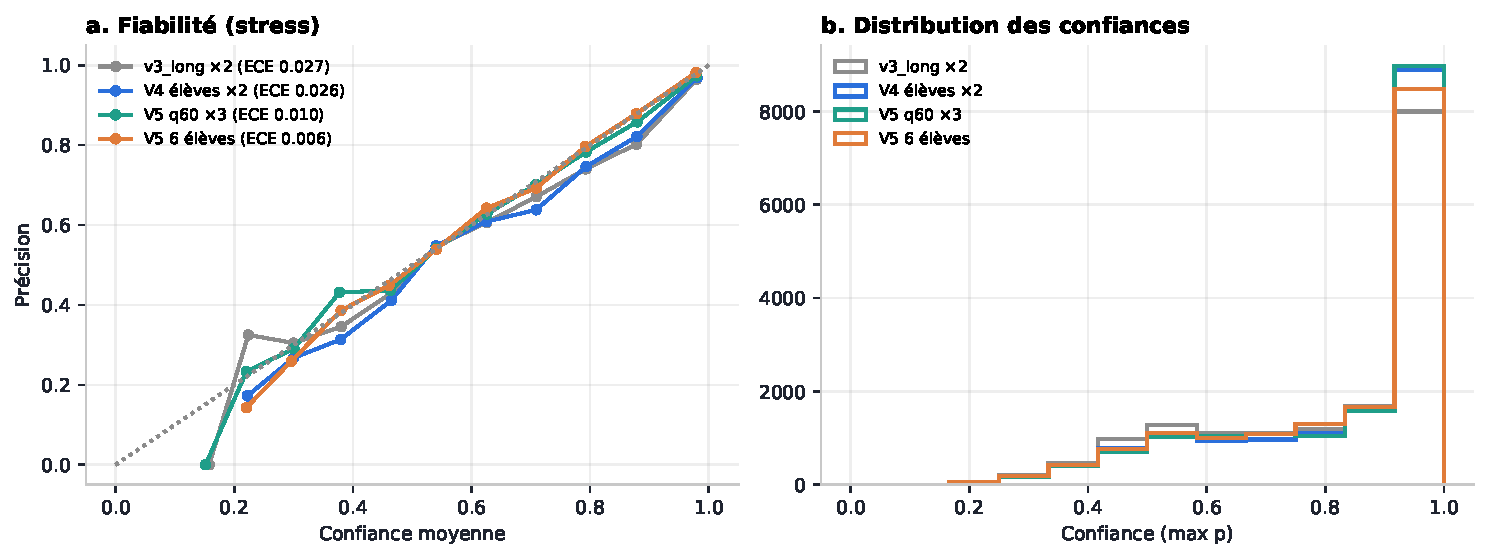
\includegraphics[width=\linewidth]{figures/v5_calibration_all.pdf}
\caption{Calibration sur le stress. (a) Courbes de fiabilité et erreur de calibration attendue (ECE, 12 classes de confiance). (b) Distribution des confiances.}
\label{fig:calib}\end{figure}

\subsection{Où se trouvent les erreurs restantes}
\begin{figure}[H]\centering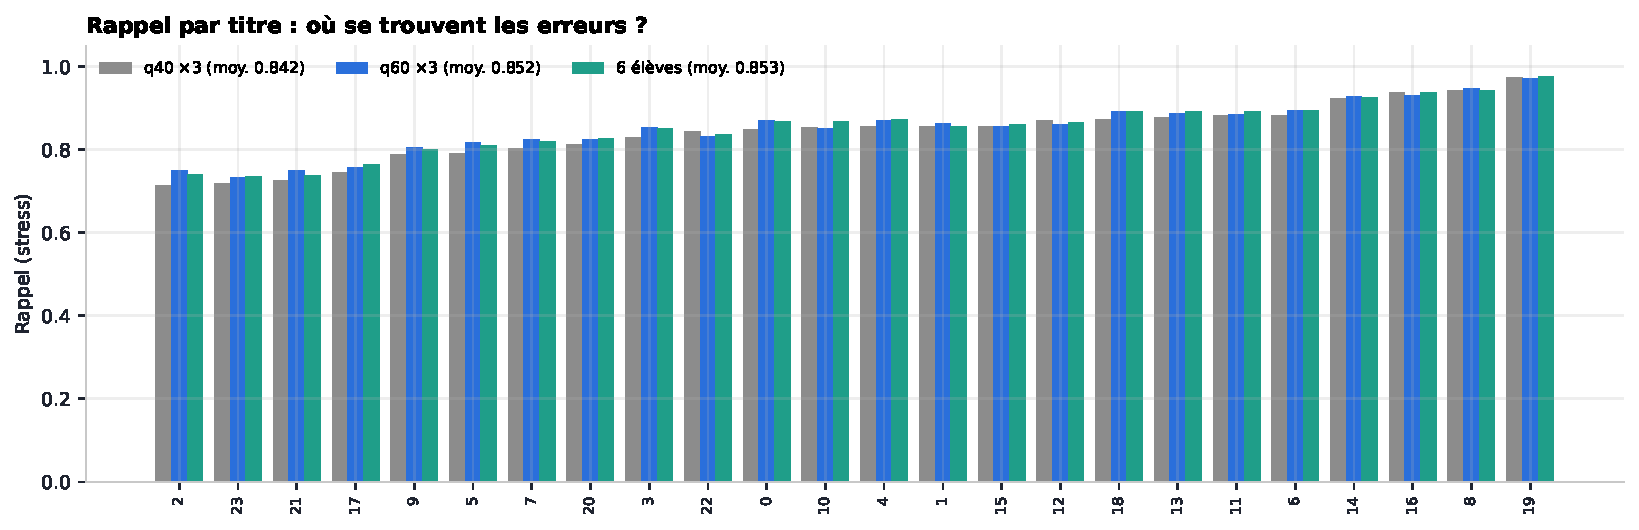
\includegraphics[width=\linewidth]{figures/v5_recall_by_class.pdf}
\caption{Rappel par titre sur le stress, pour les élèves q40, q60 et l'ensemble des 6, titres triés du plus difficile au plus facile.}
\end{figure}
\begin{figure}[H]\centering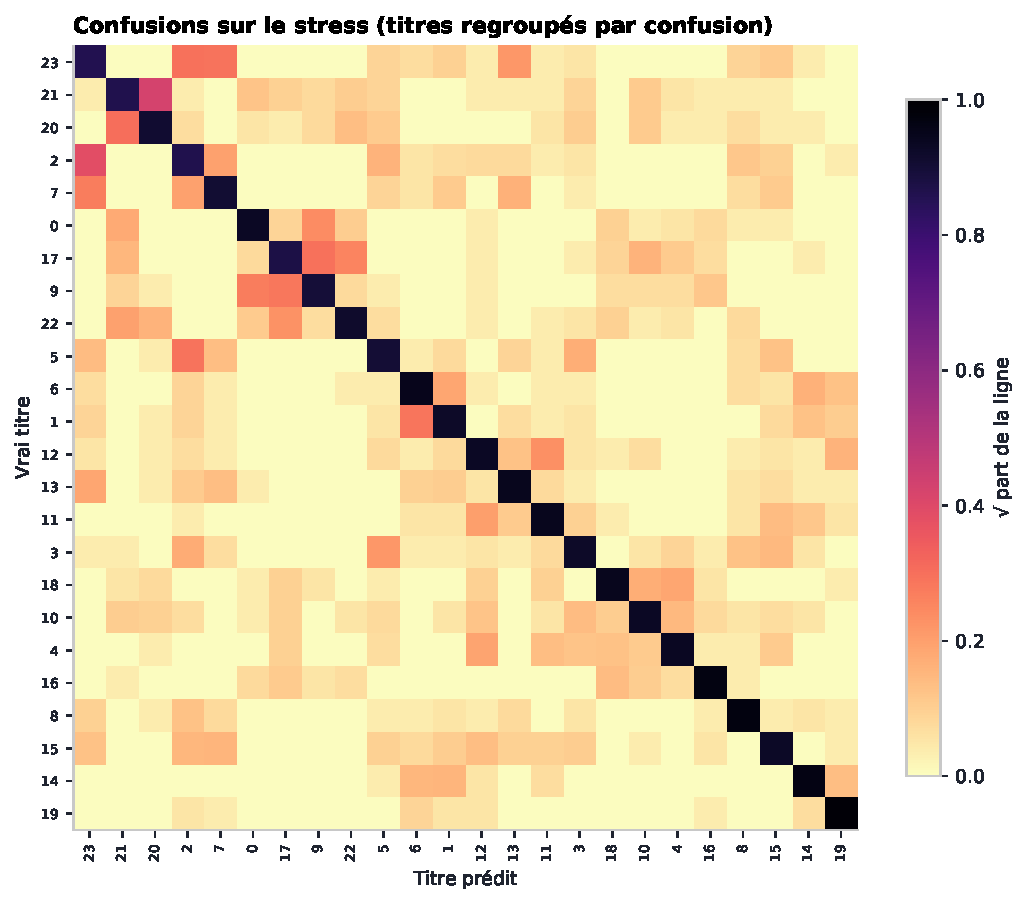
\includegraphics[width=.72\linewidth]{figures/v5_confusion.pdf}
\caption{Confusions de l'ensemble V5 sur le stress, avec les titres ordonnés par regroupement hiérarchique. Les erreurs ne sont pas diffuses : elles se concentrent dans quelques familles, notamment $\{20,21\}$, $\{2,7,23\}$, $\{0,9,17,22\}$ et $\{1,6\}$. À l'intérieur d'une famille, les titres partagent vraisemblablement un régime de tick et des conventions de lot proches (section~\ref{sec:unites}). La séparation demande alors des traits plus fins que la grille de prix.}
\label{fig:confusion}\end{figure}
\begin{figure}[H]\centering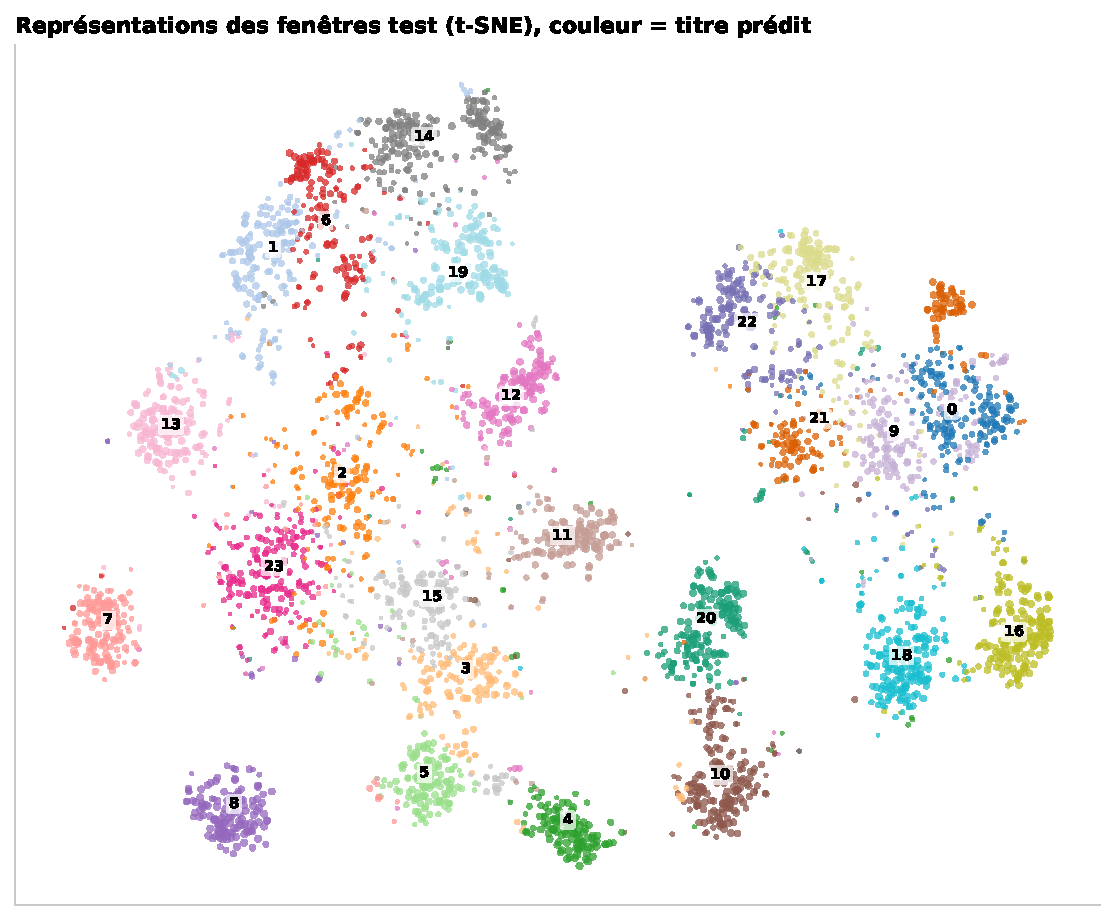
\includegraphics[width=.68\linewidth]{figures/v5_tsne_test.pdf}
\caption{Carte t-SNE de 4\,000 fenêtres test (représentations des élèves V5 refit), couleur = titre prédit, taille = confiance. Plusieurs titres forment des îlots isolés (7, 8, 13, 16). D'autres se touchent, et ce sont les mêmes familles que sur la matrice de confusion : $\{0,9,17,21,22\}$ à droite, $\{1,6,14,19\}$ en haut.}
\end{figure}

\subsection{Lecture d'ensemble}
\begin{enumerate}
\item \textbf{L'auto-apprentissage est le levier qui transfère le mieux.} Deux tours : $+2{,}0$ puis $+2{,}8$ points. Le second tour rapporte \emph{plus} que le premier, alors que son gain interne est plus petit ($+0{,}8$ point en stress équilibré). Les rendements ne décroissent pas encore.
\item \textbf{Les mesures internes sous-estiment tout ce qui exploite la période test.} C'était déjà le cas des voisins ($+1{,}3$ en interne, $+3{,}2$ au LB). Valid et stress appartiennent à la période d'entraînement : elles ne contiennent pas la direction du changement de période, qui est justement ce que les élèves apprennent.
\item \textbf{Le protocole de contrôle a été décisif.} Sans la soumission D, le $+2$ de la V4 aurait été attribué en partie aux 90 époques, qui en réalité \emph{coûtent} des points. Une soumission, une différence : c'est ce qui rend les conclusions défendables.
\item \textbf{Règle d'arrêt.} Le biais de confirmation grandit à chaque tour. Un troisième tour (professeur V5 ALL) n'est justifié que tant que le LB progresse. Le premier tour sans gain arrête la boucle.
\end{enumerate}
